\section{Method}

Given multi-view videos of a user with some arbitrary motions, our goal is to reconstruct a relightable and animatable avatar of the user.
The key challenge of this task is disentangling the geometry, material of the clothed body, and lighting, which is a highly ill-posed problem. 
To tackle this problem, we first reconstruct the body geometry from the input videos using the neural rendering techniques, where the geometry is modeled by a neural signed distance function (SDF) field and 
the dynamics of the human body are modeled with a rigid bone transformation of SMPL~\cite{loper2015smpl} model plusing an invertible neural deformation field (Sec.\ref{sec:geo_rec}, top left of Fig.\ref{fig:pipeline}).
Then, with the reconstructed geometry, we train a pose-aware part-wise light visibility estimation network, which is able to predict the light visibility of any query point under any light direction and body pose (Sec.\ref{sec:vis_est}, bottom left of Fig.\ref{fig:pipeline}).
Finally, with the visibility information, we achieve the disentangling of the material of the human body and the illumination parameters (Sec.\ref{sec:mat_est}, top right of Fig.\ref{fig:pipeline}).
Therefore, we can render a free-viewpoint video of the human with any target pose and illumination. 

\subsection{Geometry and Motion Reconstruction}
\label{sec:geo_rec}
Dynamic body deformation consists of articulated rigid motion and neural non-rigid deformation.
Correspondingly, we propose a mesh-based inverse skinning method and an invertible neural deformation field to map points between the canonical and the observation space bidirectionally.

\textbf{Mesh-based Inverse Skinning.}
The rigid motion is computed using linear blend skinning (LBS) algorithm \cite{pose_deformation}.
For point $\mathbf{x}_c$ in the canonical space, we use the bone transformation matrices $\{\mathbf{B}_b\}^{24}_{b=1}$ of the SMPL~\cite{loper2015smpl} model to transform $\mathbf{x}_c$ to $\mathbf{x}_o$ in the observation space (we omit the transformations of homogeneous coordinates for simplicity of notation):
\begin{equation}
    \mathbf{x}_o = \sum_{b=1}^{24} \left( w_b(\mathbf{x}_c) \mathbf{B}_b \right) \mathbf{x}_c
\end{equation}
where $w_b(\mathbf{x}_c)$ is the skinning weights of $\mathbf{x}_c$, and $\sum_{b=1}^{24} w_b(\mathbf{x}_c) = 1$.
Similarly, for $\mathbf{x}_o$ in the observation space, we can transform it back to the canonical space by:
\begin{equation}
    \mathbf{x}_c = \sum_{b=1}^{24} \left( w_b(\mathbf{x}_o) \mathbf{B}_b \right)^{-1} \mathbf{x}_o
\end{equation}
Similarly, for a query view direction $\mathbf{\omega}_o$ in the observation space, we can apply the same backward transformation to get the view direction $\mathbf{\omega}_c$ in the canonical space.

In volume rendering, we need to transform sampled ray points in the observation space to the canonical space (i.e. solve the inverse skinning problem) to query their SDF and color values.
However, determining the skinning weights of points in the observation space is non-trivial as $w_b$ is calculated in the canonical space rather than the observation space.
Many existing works, such as \cite{animatablenerf, peng2022animatable, humannerf}, rely on the posed SMPL mesh and use the skinning weights of neighboring SMPL mesh points to compute the inverse skinning weights of the ray points.
However, the naked SMPL mesh differs from the body surface, resulting in inaccurate weights.
Differently, we leverage the extracted explicit body mesh to compute the inverse skinning weights.
We first extract an explicit mesh of the body in the canonical space and compute the skinning weights of mesh vertices. 
Then, we use the LBS algorithm to deform the mesh to the observation space.
For any points in the observation space, we compute their skinning weights by the skinning weights of the nearest neighbor on the deformed body mesh.
As the deformed body mesh fits the actual body surface better than the naked SMPL mesh, our method does not suffer from the inaccuracies of skinning weights.

\textbf{Invertible Deformation Field.}
Since only rigid bone transformation is not enough for modeling the body motion, we use an invertible neural displacement field to model the non-rigid motions. 
As shown in Fig.\ref{fig:pipeline}, on the one hand, we apply non-rigid motion to the explicit mesh in canonical space.
On the other hand, for sampled ray points in observation space, we need to map them back to the canonical space.
Therefore, the neural displacement field should be able to transform points bidirectionally and ensure the cycle consistency of the transformation.
So, we involve an invertible neural network to represent the non-rigid motion. 
For a point $\mathbf{x} = \left[u, v, w\right]$ in the canonical space, we use the invertible network $D$ to apply displacement to it: 
\begin{equation}
    \mathbf{x}' = D(\mathbf{x}) = \left[u', v', w'\right]
\end{equation}
Besides, the invertible network $D$ can also transform $\mathbf{x}'$ back while keep the cycle consistency:
\begin{equation}
    \mathbf{x} =  D^{-1}(\mathbf{x}') = D^{-1}(D(\mathbf{x}))
\end{equation}
To keep the cycle consistency, we design a network similar to Real-NVP \cite{real-nvp}.
Specifically, we split the coordinates $[u, v, w]$ into two parts, for example, $[u, v]$ and $[w]$. 
During forward deformation, we assume the displacement of $[w]$ is decided by the value of $[u, v]$: 
\begin{equation}
    [w'] = [w] + f([u, v])
\end{equation}
and then the displacement of $[u, v]$ is decided by $[w']$:
\begin{equation}
    [u', v'] = [u, v] + g([w'])
\end{equation}
With this two-step forward deformation $D$, we can directly get an invertible backward deformation $D^{-1}$ which deforms point $[u', v', w']$ to $[u, v, w]$ as follows:
\begin{equation}
\begin{aligned}
    [u, v] & = [u', v'] - g([w']) \\
    [w] & = [w'] - f([u, v])
\end{aligned}
\end{equation}
The functions $f(\cdot), g(\cdot)$ are implemented as MLPs, they form a transformation block of the invertible network $D$.
As the aforementioned $f(\cdot)$ makes the deformation decided by $[u, v]$ only, we stack more transformation blocks and change the split of $[u, v, w]$ in these blocks. 
We assume that the non-rigid deformations are pose-dependent, for the $i$th frame, we use the body pose $\theta_i$ as the condition of the network $D$. 
Besides, we found that it is hard to learn the deformation using only the pose and coordinates as conditions.
Thus, we use the skinning weights of the query points $\mathbf{W}(\mathbf{x})\ \in \mathbb{R}^{24}$ as an additional condition, which leads to better results.
The displacement field $D$ can be formulated as $\mathbf{x}' = D(\mathbf{x}, \theta_i, \mathbf{W}(\mathbf{x}))$.
The use of skinning weights will slightly affect the cycle consistency of the deformation network, as $\mathbf{W}(\mathbf{x})$ is not strictly equal to $\mathbf{W}(\mathbf{x}')$.
But we found the skinning weights field in the canonical pose is smooth, and the deformations are relatively small, so they are almost the same, the sacrifice on cycle consistency is negligible.
% For more details please refer to the supplemental document.

%%%%%%%%% 网络训练与Loss函数
\textbf{Network Training.}
To supervise these neural fields with videos, we use the technique proposed in VolSDF \cite{volsdf} to convert the SDF values to density and conduct volume rendering. 
% The neural color field $C$ takes query view direction, the output feature of the SDF network $G$ and normal as input.
For the color field, we introduce learnable per-frame appearance latent codes $\{l_i\}_{i=1}^N$ to model the dynamic appearance, where $N$ is the number of frames.
Besides, we optimize the pose vectors $\{\theta_i\}_{i=1}^N$, as the initial poses may not be accurate.
In sum, the training parameters contain the SDF network, the color network, the deformation network $D$, the appearance latent codes $\{l_i\}_{i=1}^N$ and the pose vectors $\{\theta_i\}_{i=1}^N$. 
The training loss consists of rendering photometric loss and multiple regularizers:
\begin{equation}
    \mathcal{L} = \lambda_{\text{pixel}}\mathcal{L}_{\text{pixel}} + \lambda_{\text{mask}}\mathcal{L}_{\text{mask}} + \lambda_{\text{eik}}\mathcal{L}_{{\text{eik}}} + \lambda_{\text{disp}}\mathcal{L}_{{\text{disp}}}
\end{equation}
where $\mathcal{L}_{\text{pixel}}$ is an L2 pixel loss for predicted color, $\mathcal{L}_{\text{mask}}$ is a binary cross-entropy loss for the rendering object mask and input mask, $\mathcal{L}_{{\text{eik}}}$ is the Eikonal regularization term \cite{eik}, $\mathcal{L}_{{\text{disp}}}$ is an L2 regularizer for the output displacements.
% During training, we extract the explict body mesh in canonical space every $k$ epoches. 
For more details about network architecture and training, please refer to the supplemental document.

\subsection{Part-wise Light Visibility Estimation}
\label{sec:vis_est}
%%%%%%%%%% 可见性估计的作用和问题定义
With the reconstructed geometry, we then conduct pose-aware light visibility estimation.
Modeling the visibility allows for the extraction or generation of shadows on images, which helps to better disentangle material and lighting from input images as well as produce physically plausible shadow effects in rendered images.
Given a query point $\mathbf{x}$ and a query light direction $\mathbf{\omega}$, our goal is to train a network to predict whether the query point will be lighted or occluded by the body in a certain a pose and light direction.

%%%%%%%%%% 前人如何处理可见性估计(静态场景重光照和Relighting4D),问题难点
Traditionally, estimating light visibility is solved by performing ray tracing.
However, for implicit neural network-based methods, tracing a path of light requires numerous queries, as we need to trace all possible lighting directions for one 3D point, which is very time-consuming.
Thus, existing methods \cite{NeRFactor, InvRender, Relighting4D} use MLPs to re-parameterize and speed up this process as $V\left(\mathbf{x}, \mathbf{\omega}\right) \mapsto v$, where $v=1$ indicates the point is visible to the light from $\omega$ direction.
However, with the motion of the human body, light visibility changes dramatically.
Relighting4D \cite{Relighting4D} leverages temporally-varying latent codes to model these changes, but it is limited to seen poses as there is no latent code for unseen motions.
To solve this problem, we need to make it pose-aware for light visibility estimation.
A naive approach is to use the pose vectors as the condition of the visibility network, but we found this approach does not work well as the relationship among pose, lighting, and shadow is too complex to be modeled.

%%%%%%%%%% 我们的方法,分块估计的motivation
Our observation is that how light rays are blocked is determined by the object geometry, even though the human body as a whole can be in different complex shapes caused by pose changes, for a single body part, its geometry changes are relatively small among different poses.
So, we divide the human body into $N(=15)$ parts as shown in the orange rectangle in Fig.\ref{fig:pipeline}, where different colors denote different body parts.
Then for each body part, we train a neural network respectively to predict how the body part blocks the lights.
Finally, we combine the light visibility of all body parts by multiplying all the predicted visibility.
Thus, our method achieves light visibility prediction of any query points, light directions, and body poses.

%%%%%%%%%% 分块估计的实现方式
To be specific, given the query point $\mathbf{x}_o$ and light direction $\mathbf{\omega}_o$ in observation space, we first transform them to the local coordinate of each body part:
\begin{equation}
    \mathbf{x}_i = \mathbf{B}_i^{-1} \mathbf{x}_o, \quad \mathbf{\omega}_i = \mathbf{B}_i^{-1} \mathbf{\omega}_o
\end{equation}
where $\mathbf{B}_i$ is the bone transformation of the $i$th body part.
Besides, although the geometry changes of body parts are relatively small, there are still some pose-dependent deformations. 
And the geometry of a body part is majorly affected by the poses of its neighboring joints, so we use them as the networks' condition.
We denote the neighboring joints of body part $i$ as $J(i)$.
So, the visibility network of a body part $i$ can be formulated as:
\begin{equation}
    V_i\left(\mathbf{x}_{i}, \mathbf{\omega}_{i}, \mathbf{\theta}_{J(i)}\right) \mapsto v_i
\end{equation}

For network training, we sample different query points, light directions, and body poses, then we perform ray tracing to compute the ground truth light visibility of each body part.
We impose binary cross-entropy loss to train the networks for visibility estimation.


\subsection{Material and Light Estimation}
\label{sec:mat_est}
%%%%%%%%%% 材质光照估计概览,输入输出定义,介绍材质光照模型
At this stage, we fix the geometry and light visibility estimation modules and optimize the material network and light parameters as shown in the green rectangle in Fig.\ref{fig:pipeline}.
Here, we parameterize the material using the Disney BRDF \cite{disneyBRDF} model and use albedo and roughness to represent the material.
However, we found that directly optimizing the roughness is difficult.
Similar to \cite{zhuo17, li22, psnerf}, we use a weighted combination of specular bases.
Each basis is defined by a different roughness value.
For a query point in the canonical space, we use an implicit neural network $M$ to predict its albedo value and roughness weights.
For environment light, we parameterize it using $L=128$ spherical Gaussians (SGs) \cite{SG}:
\begin{equation}
    E\left(\mathbf{\omega}_{i}\right)=\sum_{j=1}^L G\left(\mathbf{\omega}_{i} ; \mathbf{\xi}_j, \lambda_j, \mathbf{\mu}_j\right)
\end{equation}
where $\mathbf{\omega}_i\in \mathbb{S}^2$ is the query lighting direction, $\mathbf{\xi}_j\in \mathbb{S}^2$ is the lobe axis, $\lambda_j \in \mathbb{R}_{+}$ is the lobe sharpness, $\mu_j \in \mathbb{R}^3$ is the lobe amplitude. 
To compute the visibility of an SG light, we sample 4 directions around the lobe axis based on the distribution defined by $\lambda_j$. 
Then we predict their visibilities by the trained light visibility estimation network and use the weighted sum of these samples as the visibility of the SG light.

%%%%%%%%%% 渲染方法
With geometry, material, environment light, and light visibility, we can render images of the human body using a differentiable renderer.
The rendering equation computes the outgoing radiance $L_o$ at point $\mathbf{x}$ viewed from $\mathbf{\omega}_o$:
\begin{equation}
    L_o\left(\mathbf{x}, \mathbf{\omega}_o\right)=\int_{\Omega} L_{i }\left(\mathbf{x}, \mathbf{\omega}_i\right) R\left(\mathbf{x}, \mathbf{\omega}_i, \mathbf{\omega}_o, \mathbf{n}\right)\left(\mathbf{\omega}_i \cdot \mathbf{n}\right) \mathrm{d} \mathbf{\omega}_i
\end{equation}
where $L_{i}\left(\mathbf{x}, \mathbf{\omega}_i\right)$ is the incident radiance of point $\mathbf{x}$ from direction $\mathbf{\omega}_i$, which is determined by the environment light $E$ and masked by the light visibility. 
$R\left(\mathbf{x}, \mathbf{\omega}_i, \mathbf{\omega}_o, \mathbf{n}\right)$ is the Bidirectional Reflectance Distribution Function (BRDF) which is determined by the albedo values and roughness weights predicted by $M$. 

%%%%%%%%%% 训练方式与Loss函数
To train the material network $M$ and the light parameters of $E$, we use L1 pixel loss between the rendered images and the recorded images.
However, there are strong ambiguities in solving material and lighting, so we apply some regularization strategies.
First, the material network is designed as an encoder-decoder architecture following \cite{InvRender}, so that we can impose constraints on the latent space to ensure the sparsity of albedo and roughness weights. 
We denote the encoder and decoder of $M$ as $M_E$ and $M_D$, for a query point $\mathbf{x}$ in the canonical space, its latent vector is $\mathbf{z} = M_E(\mathbf{x}) \in \mathbb{R}^N$. 
For $K$ latent codes in a batch $\{\mathbf{z}_i\}_{i=0}^K$, we impose Kullback-Leibler divergence loss to encourage the sparsity of the latent space:
\begin{equation}
    \mathcal{L}_{\text{kl}} = \sum_{j=1}^N \mathrm{KL}\left(\rho || \hat{\rho}_j\right)
\end{equation}
where $\hat{\rho}_j$ is the average of the $j$th channel of $\{\mathbf{z}_i\}_{i=0}^K$, $\rho$ is set to 0.05.
Moreover, we apply smooth loss to both the latent vectors and the output albedo and roughness weights by adding perturbations:
\begin{equation}
\begin{aligned}
    \mathcal{L}_{\text{smooth}} = & \lambda_\mathbf{z} \|M_D(\mathbf{z}) - M_D(\mathbf{z} + \mathbf{\xi}_\mathbf{z})\|_1 + \\ 
    & \lambda_\mathbf{x} \| M(\mathbf{x}) - M(\mathbf{x} + \mathbf{\xi}_\mathbf{x})\|_1
\end{aligned}
\label{eq:lsmooth}
\end{equation}
where $\mathbf{\xi}_\mathbf{z}$ and $\mathbf{\xi}_\mathbf{x}$ are the perturbations of the latent code $\mathbf{z}$ and the query point $\mathbf{x}$, which is sampled from a Gaussian distribution with zero mean and 0.01 variance.

In sum, the full training loss for this stage is:
\begin{equation}
    \mathcal{L} = \lambda_{\text{pixel}} \mathcal{L}_{\text{pixel}} + \lambda_{\text{kl}} \mathcal{L}_{\text{kl}} + \lambda_{\text{smooth}} \mathcal{L}_{\text{smooth}}
    \label{eq:lmat}
\end{equation}

With the trained geometry field, the deformation field, the light visibility estimation networks $V$, and the material network $M$, we can render the avatar in novel poses, lightings, and viewpoints. 
Thus we achieve a relightable and animatable neural avatar. 



\begin{table*}[t]
\begin{center}
\scalebox{0.9}{
\begin{tabular}{cccccccccc}
\hline
\multirow{2}{*}{Method} & \multicolumn{3}{c}{Albedo Map} & \multicolumn{3}{c}{Relighting (Training poses)} & \multicolumn{3}{c}{Relighting (Novel poses)} \\
                        & PSNR$\uparrow$ & SSIM$\uparrow$ & LPIPS$\downarrow$ & PSNR$\uparrow$ & SSIM$\uparrow$ & LPIPS$\downarrow$ & PSNR$\uparrow$ & SSIM$\uparrow$ & LPIPS$\downarrow$  \\
\hline
Relighting4D~\cite{Relighting4D} & 21.5103 & 0.8320 & 0.2299 & 19.7323 & 0.7568 & 0.2721 & 16.7475 & 0.6729 & 0.3330 \\
\hline
Ours w/o visibility & 24.7611 & 0.8918 & 0.1655 & 23.7758 & 0.8376 & 0.2223 & 18.9768 & 0.7333 & 0.2638 \\
Ours w/o part-wise visibility & \textbf{25.2150} & \textbf{0.8921} & 0.1652 & 24.7064 & 0.8462 & 0.2173 & 19.7119 & 0.7452 & 0.2580 \\
Ours & 25.1666 & 0.8919 & \textbf{0.1645} & \textbf{25.3477} & \textbf{0.8546} & \textbf{0.2124} & \textbf{19.8622} & \textbf{0.7518} & \textbf{0.2533} \\
\hline
\end{tabular}
}
\caption{Quantitative comparison of the reconstructed albedo and the relighting results on synthetic data.}
\label{tab:syn}
\end{center}
\end{table*}

\begin{figure}[t]
\begin{center}
   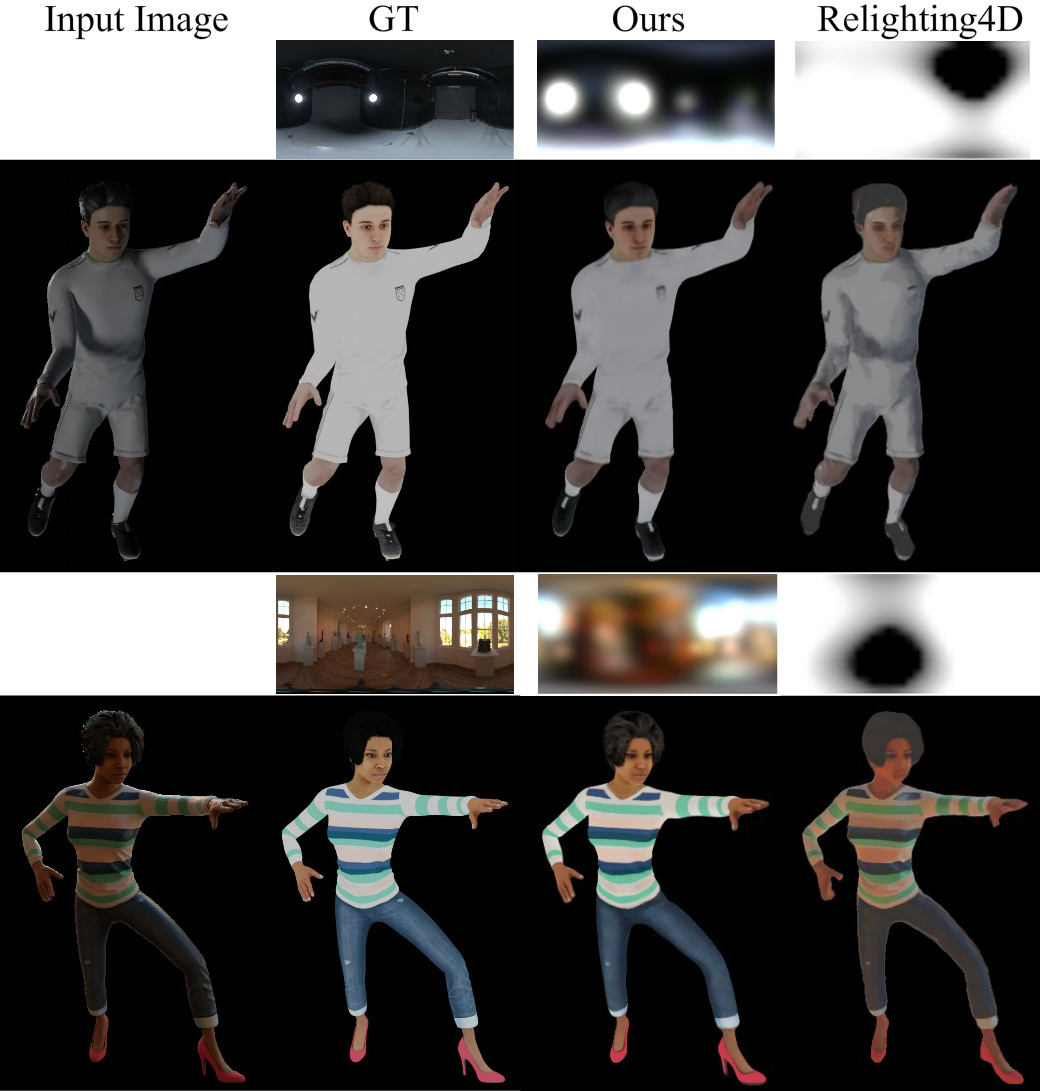
\includegraphics[width=1.0\linewidth]{./fig/albedo_rec.jpg}
\end{center}
\caption{Qualitative comparison of the reconstructed albedo and lighting on synthetic data. Environment lighting is shown on top of the albedo in each result.}
\label{fig:albedo_rec}
\end{figure}

\begin{figure}[t]
\begin{center}
   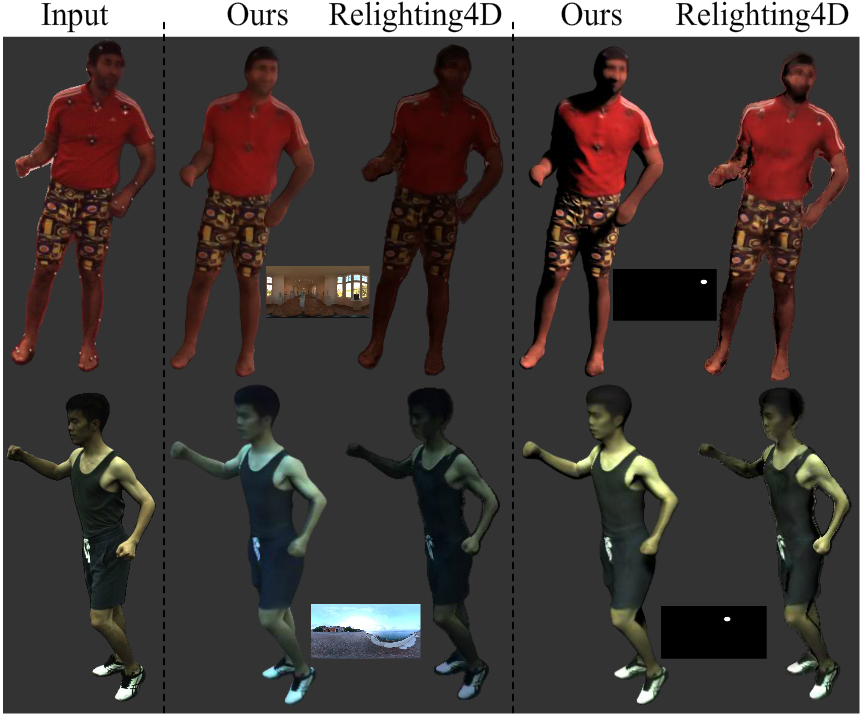
\includegraphics[width=1.0\linewidth]{./fig/relit_real.jpg}
\end{center}
\caption{Qualitative comparison of relighting results on real data. The environment lighting of the rendered results is shown at the bottom.}
\label{fig:relit_real}
\end{figure}
